% --------------------------------------------------------------------------- %
\chapter{Measurement and Data Processing}
\label{chap:measurementProcess}
% --------------------------------------------------------------------------- %

\todo[inline]{%
    Primary questions to answer in this chapter: What did we measure, how, and
    why?
}

The  goal in this project was to create an efficient, streamlined workflow for
measuring  multiple  sensor  chips  and  correlating the results in meaningful
ways.  The  conclusions  drawn  in  this  report  mostly  originated  from  DC
measurements; A known voltage is applied to the chip's input and its output is
observed  in  function  of  the  preamp gain, the sampling frequency $fs$  and
different chips. output-to-input voltage

\begin{figure}[t]
    \centering
    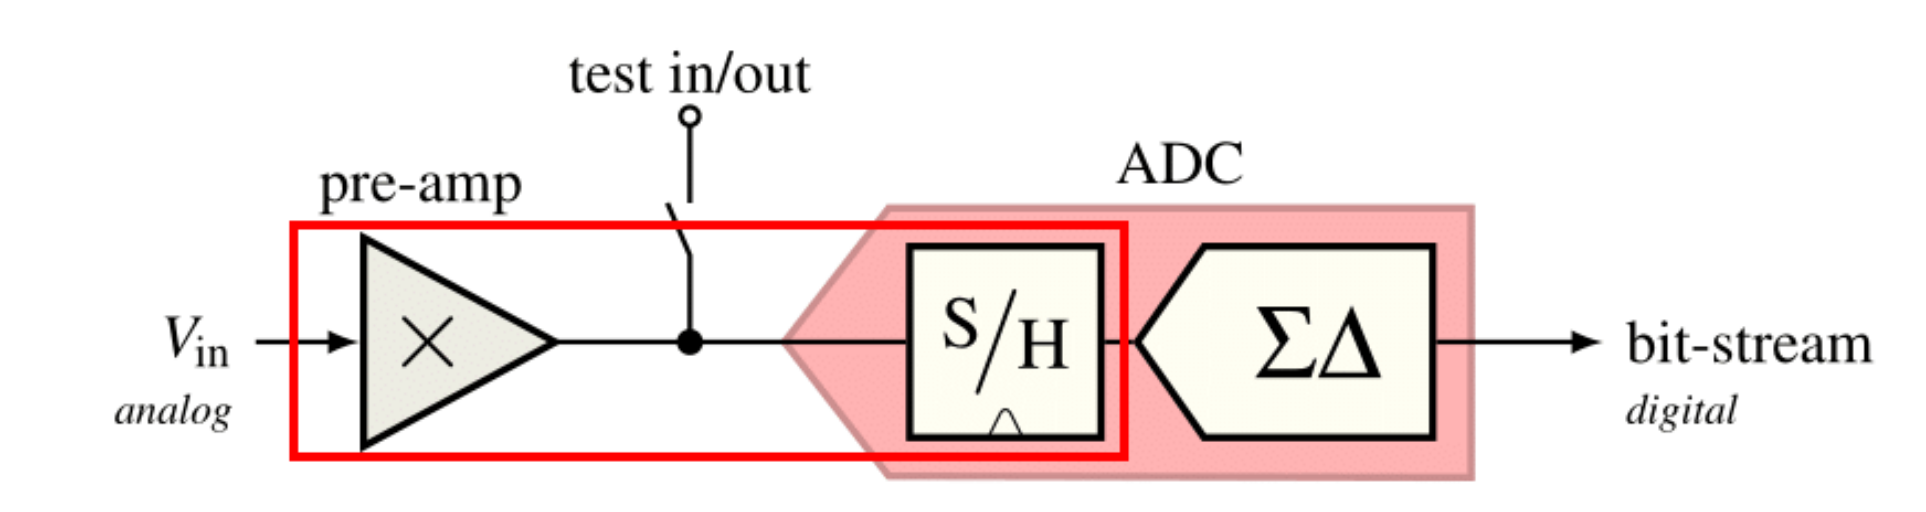
\includegraphics[width=.8\linewidth]{images/blockdiagram.png}
    \caption{Rough block diagram of the sensor chip}
    \label{fig:blockdiagram}
\end{figure}



Two different  kinds  of  measurements were performed: Analog measurements were
used to assess the performance of the  preamp  via  the \signal{TEST OUT} pin.
Secondly, digital measurements for assessing the $\Sigma\Delta M$  as  well as
the  two  components  combined  are  derived  by  evaluating the  bit  stream.

Analog measurement data  is captured with an osccilloscope  and then evaluated
on a PC. The bit stream is captured and processed on the \raspi.

For both the  preamp as well as the $\Sigma\Delta$  modulator, DC measurements
over an input  voltage range between \SI{0.5}{\volt}  and  \SI{2.5}{\volt} are
performed. AC measurements are used to assess the system's frequency behavior.

Both DC and AC measurements are performed with various settings for the preamp
(sign,  gain,  on/off)  as  well as  the  $\Sigma\Delta$  modulator  (sampling
frequency).

The sample size is 10 chips, unless indicated otherwise.

Based on these measurements and their  analysis in the next chapter, we strive
to answer the question  of what sort of use cases this  sytem is suitable for,
and with which settings.

% TODO: noise
% TODO: resolution in bits under a given set of circumstances
% TODO: Measurement methodology


% --------------------------------------------------------------------------- %
\section{Pre-Amplifier: DC Measurements}
\label{sec:preAmpDC}
% --------------------------------------------------------------------------- %

% --------------------------------------------------------------------------- %
\section{Sigma-Delta Converter: DC Measurements}
\label{sec:sigdelDC}
% --------------------------------------------------------------------------- %

% --------------------------------------------------------------------------- %
\section{Complete System: DC Measurements}
\label{sec:systemDC}
% --------------------------------------------------------------------------- %

% --------------------------------------------------------------------------- %
\section{Pre-Amplifier: AC Measurements}
\label{sec:preAmpAC}
% --------------------------------------------------------------------------- %

% --------------------------------------------------------------------------- %
\section{Sigma-Delta Converter: AC Measurements}
\label{sec:sigdelAC}
% --------------------------------------------------------------------------- %

% --------------------------------------------------------------------------- %
\section{Complete System: AC Measurements}
\label{sec:systemAC}
% --------------------------------------------------------------------------- %
